\documentclass{article}
\usepackage{graphicx}
\usepackage[dot, autosize, outputdir="graphfiles/"]{dot2texi}
\usepackage{tikz}
\usepackage{amsmath, mathtools}
\usetikzlibrary{shapes}
\begin{document}
\section{DFA Minimisation}
In this assignment we are asked to minimise \ref{dfatomin} in accordance to the minimisation steps presented in the lecture. Unfortunately I was unable to attend the lecture, but from the lecture slides, it appears that the method specified in the book was followed.\\

\begin{figure}[h]
\begin{center}
	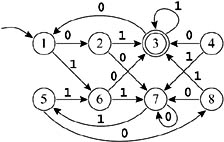
\includegraphics{dfatominimise.png}
	\caption{DFA to minimise}
	\label{dfatomin}
\end{center}
\end{figure}

In order to minimise this DFA we need to identify the different groups, check them and mark them accordingly. The first thing we do is create a subset of our nodes without accepting nodes \(S\\F={1,2,4,5,6,7,8}\) and a set of our accepting nodes \(F={3}\).\\
Being that there is only one node in our set \(G1=F\) we know that this group is consistent and can mark it without checking it. We name our set \(G2=S\\F\). Now we wish to check this group for consistency. Upon an inspection of the DFA we can conclude that there are no dead groups.\\
\begin{table}[h]
	\begin{center}
		\begin{tabular}{|l|c|r|}
			\hline
			G2 & 0 & 1\\\hline
			1 & G2 & G2\\\hline
			2 & G2 & G1\\\hline
			4 & G1 & G2\\\hline
			5 & G2 & G2\\\hline
			6 & G1 & G2\\\hline
			7 & G2 & G2\\\hline
			8 & G2 & G1\\\hline
		\end{tabular}
	\caption{Checking G2 for consistency}
	\end{center}
\end{table}

This group is obviously not consistent, so we split it into groups of that are maximally consistent. By maximally consistent groups, we mean that we split \(G2\) into, in this case two, groups that are seemingly consistent. As we do this all marked groups are unmarked and checked again. \(G1\) is still a singleton group and thus still consistent and we can mark it. \(G2\) is split into the groups \(G3={1,5,7}\), \(G4={2,8}\), and \(G5={4,6}\). We then check if \(G3\) is consistent.

\begin{table}[h]
	\begin{center}
		\begin{tabular}{|l|c|r|}
			\hline
			G3 & 0 & 1\\\hline
			1 & G4 & G5\\\hline
			5 & G4 & G5\\\hline
			7 & G3 & G3\\\hline
		\end{tabular}
	\caption{Checking G3 for consistency}
	\end{center}
\end{table}

Obviously \(G3\) isn't consistent, so it is further split into two group \(G6={1,5}\) and \(G7={7}\).
\begin{table}[h]
	\begin{center}
		\begin{tabular}{|l|c|r|}
			\hline
			G6 & 0 & 1\\\hline
			1 & G4 & G7\\\hline
			5 & G4 & G7\\\hline
		\end{tabular}
	\caption{Checking G6 for consistency}
	\end{center}
\end{table}

\(G6\) is consistent, so we add it to our set of consistent groups \(S={G1, G6}\).\\
\begin{table}[h]
	\begin{center}
		\begin{tabular}{|l|c|r|}
			\hline
			G4 & 0 & 1\\\hline
			2 & G7 & G1\\\hline
			8 & G7 & G1\\\hline
		\end{tabular}
	\caption{Checking G4 for consistency}
	\end{center}
\end{table}
\(G4\) is consistent, so we add it to the set of consistent groups \(S={G1, G6, G4}\).\\
\begin{table}[h]
	\begin{center}
		\begin{tabular}{|l|c|r|}
			\hline
			G5 & 0 & 1\\\hline
			4 & G1 & G7\\\hline
			6 & G1 & G7\\\hline
		\end{tabular}
	\end{center}
	\caption{Checking G5 for consistency}
	\label{g5-check}
\end{table}
\(G5\) is consistent (see table \ref{g5-check}), so we add it to the set of consistent groups \(S={G1, G6, G4, G5}\).\\
Being that \(G7\) is a singleton group, this is consistent so we can add it to our set of consistent groups \(S={G1, G6, G4, G5, G7}\) and thus we are done as there are no more unmarked groups.\newpage
The minimised DFA will then look as follows: 

\begin{dot2tex}
digraph {
	rankdir=LR;
	node [shape=circle];
	start [color=white, shape=point]
	G1 [label="G1", shape=doublecircle]
	G4 [label="G4"]
	G5 [label="G5"]
	G6 [label="G6"]
	G7 [label="G7"]
	start -> G6;
	G6 -> G4 [label="0"]
	G6 -> G5 [label="1"]

	G4 -> G1 [label="0"]
	G4 -> G7 [label="1"]

	G1 -> G6 [label="0"]
	G1 -> G1 [label="1"]

	G5 -> G7 [label="1"]
	G5 -> G1 [label="0"]

	G7 -> G6 [label="1"]
	G7 -> G7 [label="0"]
}
\end{dot2tex}
\begin{figure}[h]
	\begin{center}
		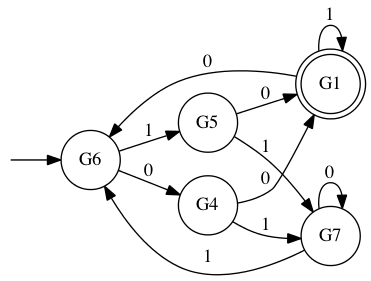
\includegraphics[scale=0.5]{graphfiles/dfamin.png}
		\caption{"Minimised DFA"}
	\end{center}
\end{figure}

\section{Backtracking Automaton}
\subsection{Give an NFA for each expression \(\alpha{1},\alpha{2},\alpha{3}\) and combined NFA}
\begin{dot2tex}[options=-t math]
digraph {
	rankdir=LR
	node [shape=circle];
	start [color=white, shape=point]
	1 [label="1"]
	2 [label="2", shape=doublecircle]
	3 [label="3"]
	4 [label="4"]

	start -> 1;	
	1 -> 2 [label="a"]
	2 -> 3 [label="\epsilon"]
	3 -> 4 [label="b"]
	4 -> 2 [label="\epsilon"]
}
\end{dot2tex}
\begin{figure}[h]
	\begin{center}
	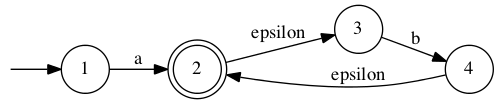
\includegraphics[scale=0.5]{graphfiles/a1.png}
	\caption{"a1 NFA"}
	\end{center}
\end{figure}

\begin{dot2tex}
digraph {
	rankdir=LR
	node [shape=circle]
	1 [label="1"]
	2 [label="2"]
	3 [label="3"]
	4 [label="4", shape=doublecircle]

	start -> 1;
	1 -> 2 [label="\epsilon"]
	2 -> 3 [label="\epsilon"]
	3 -> 2 [label="a"]
	2 -> 4 [label="b"]
}\end{dot2tex}
\begin{figure}[h]
	\begin{center}
	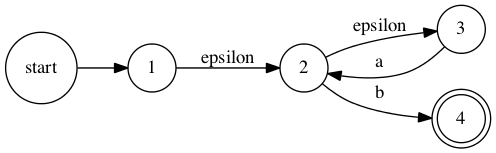
\includegraphics[scale=0.5]{graphfiles/a2.png}
	\caption{"a2 NFA"}
	\end{center}
\end{figure}
\begin{dot2tex}
digraph {
	rankdir=LR
	node [shape=circle]
	1 [label="1"]
	2 [label="2"]
	3 [label="3"]
	4 [label="4"]
	5 [label="5", shape=doublecircle]
	
	start -> 1;
	1 -> 2 [label="\epsilon"]
	2 -> 3 [label="\epsilon"]
	3 -> 4 [label="a"]
	4 -> 2 [label="b"]
	2 -> 5 [label="c"]
}\end{dot2tex}
\begin{figure}[h]
	\begin{center}
	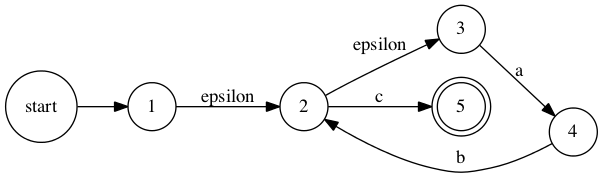
\includegraphics[scale=0.5]{graphfiles/a3.png}
	caption{"a3 NFA"}
	\end{center}
\end{figure}

\begin{dot2tex}
digraph {
	rankdir=LR
	
	1 [label="1"]
	
	start -> 1;
	
	2 [label="2"]
	3 [label="3"]
	4 [label="4"]
	5 [label="5"]
	6 [label="6"]
	7 [label="7"]
	8 [label="8"]
	9 [label="9", shape=doublecircle]

	1 -> 3 [label="a"]
	3 -> 2 [label="\epsilon"]
	2 -> 3 [label="b"]
	3 -> 9 [label="\epsilon"]
	1 -> 5 [label="\epsilon"]
	5 -> 4 [label="\epsilon"]
	4 -> 5 [label="a"]
	5 -> 9 [label="b"]
	1 -> 8 [label="\epsilon"]
	8 -> 6 [label="\epsilon"]
	6 -> 7 [label="a"]
	7 -> 8 [label="b"]
	8 -> 9 [label="c"]
}\end{dot2tex}
\begin{figure}[!htb]
	\begin{center}
	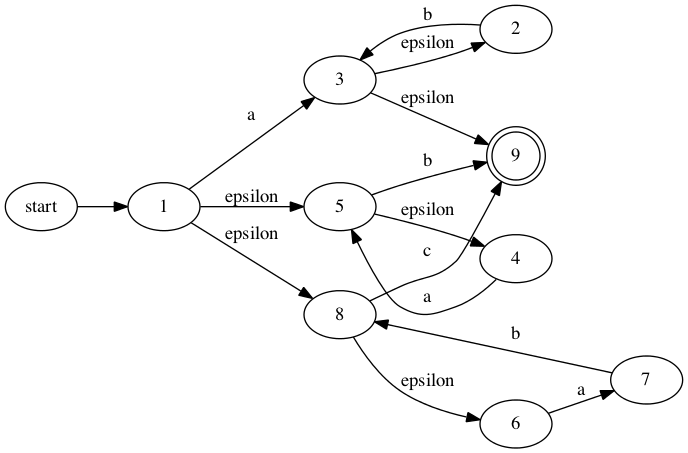
\includegraphics[scale=0.5]{graphfiles/combined.png}
	\caption{"Combined NFA"}
	\end{center}
\end{figure}
\newpage

\subsection{Convert the combined NFA into a DFA}
We want to find the inital epsilon transitions from the starting point.
\[\epsilon -closure(\{1\}) = \{1, 5, 8, 4, 6\}\]
Now we would like to find the states of the DFA, which is done by subset construction:
\[move(s_0, a) = \{2, 3, 9, 4, 5, 7\} = s_1\]
\[move(s_0, b) = \{9\} = s_2 \]
\[move(s_0, c) = \{9\} = s_3 \]
\[move(s_1, b) = \{3,2,9,8,6\} = s_4\]
\[move(s_4, c) = \{9\} = s_5\]
\[move(s_4, a) = \{7\} = s_6\]
\[move(s_6, b) = \{8, 6\} = s_7\]

\begin{dot2tex}
digraph {
	s0 [label="s0"]
	s1 [label="s1", shape=doublecircle]
	s2 [label="s2", shape=doublecircle]
	s3 [label="s3", shape=doublecircle]
	s4 [label="s4"]
	s5 [label="s5"]

	s0 -> s1 [label="a"]
	s0 -> s2 [label="b,c"]
	s1 -> s3 [label="b"]
	s1 -> s1 [label="a"]
	s2 -> s2 [label="b"]
	s3 -> s2 [label="c"]
	s3 -> s2 [label="b"]
	s3 -> s4 [label="a"]
	s4 -> s5 [label="b"]
	s5 -> s4 [label="a"]
} \end{dot2tex}
\begin{figure}[h]
	\begin{center}
	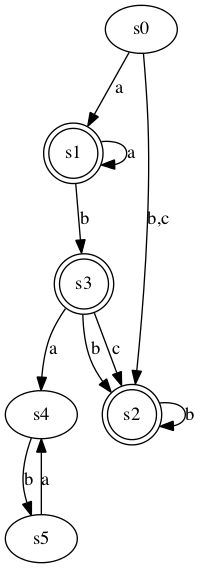
\includegraphics[scale=0.5]{graphfiles/mydfa.png}
	\caption{"Result of NFA to DFA result"}
	\end{center}
\end{figure}

\subsection{Describe the transitions and backtracking}
First we move as follows: \(s0 - s1 - s3 - s4 - s5 - s4\). However only the initial two transitions are saved, and the remaining is sent back to the input stream, thus we have currently parsed "ab".\\
Then we repeat the movement, but stop after the first time we reach \(s4\) giving us: "ab".
We then move \(s0 - s1\) after which we cannot omve futher and restart from the initial state, we have obtained "a".\\
We now move \(s0 - s2\), to obtain a "c". We do this twice, we now have "cc". Finally we move \(s0 - s1\) to obtain the final "a", thus we have now parsed the entire input "ababacca".

\section{Mosmllex scanner construction}
\section{More on regular languages and tokenization}
\subsection{Using the alphabet of decimal digits, give regular expression describing given languages}
\begin{itemize}
\item Write a regular expression describing numbers divisible by 5.\\
\([0-9]^*[0|5]^+\)
\item Write a regular expression describing numbers where the number 5 occurs exactly three times.\\
\([0-4]*[6-9]*[0-4]*5[0-4]*[6-9]*[0-4]*5[0-4]*[6-9]*[0-4]*5[0-4]*[6-9]*[0-4]*\)
\end{itemize}
\subsection{Are the following languages over the alphabet of decimal digits regular? Give short convincing reasons for your answers}
\begin{itemize}
\item Numbers which contain digit '1' exactly as many times as digit '2'.\\
It isn't a regular language, as isn't bounded, which a regular language must be.
\item Numbers N < 1.000.000 which contain digit '1' exactly as often as digit '2'.\\
Yes. It can be described as we are working with a finite sequence, and can thus implement rules, around which we build our regular expression. I have not figured out the regular expression though.
\end{itemize}
\end{document}
